%-*-coding: utf-8-*-

\chapter{Описание предложенного алгоритма}  \label{chapter2}
В данной главе будет описан предложенный алгоритм консенсуса на основе комитета участников, проведен его анализ и доказательство,
а также возможные модификации.

\section{Схема предложенного алгоритма}
В данном разделе будет описана основная схема и краеугольные камни алгоритма.

В основе алгоритма находится комитет участников сети, 
которые принимают транзакции от \textit{клиентов} - узлов, не входящих в комитет, 
и обрабатывают их.
Каждый участник комитета может быть идентифицируем некоторым образом, например, его публичным ключом, и знает идентификаторы всех остальных членов комитета.
Размер комитета равен некоторому постоянному числу $n$, которое не меняется с течением времени. 
Новый участник может присоединиться к нему, в то время как один из членов коммитета должен покинуть, чтобы размер оставался равным $n$.

Комитет ответственнен за корректное состояние хранилища и порядка операций, изменяющих его.
Если какой-то из участников хочет внести некоторое изменение в хранилище, остальные участники должны прийти к консенсусу, является ли оно корректным. 
Алгоритм, с помощью которого участники будут приходить к общему решению, является одной из важных частей решения.  
По сути, участники должны реализовывать задачу SMR(State Machine Replication)[ссылка].

Таким образом, алгоритм условно можно разбить на две составляющие: алгоритм SMR в его основе и то, каким образом новые участники попадают в комитет.

\begin{figure}[!h]
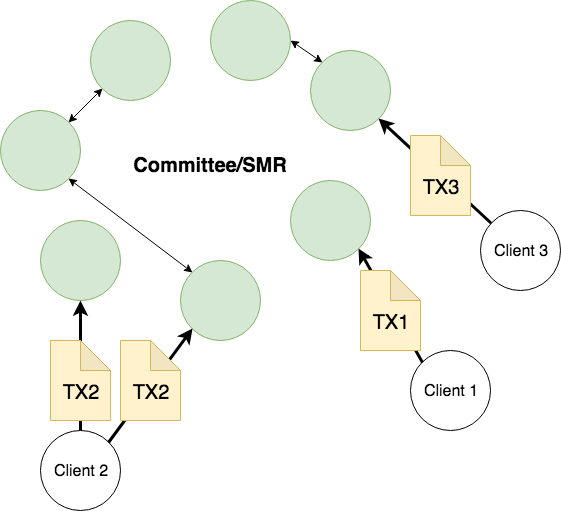
\includegraphics[scale=0.6]{Committee}
\caption{\textbf{Cхематическое изображение алгоритма}}
\label{fig:committee}
\end{figure}

\section{Рассматриваемая модель}
В данном разделе мы опишем модель, в которой работает предложенный алгоритм.

В рамках данной работы мы рассматриваем \textit{инклюзивную} (permissionless)[ссылка] модель, в которой:
\begin{itemize}
\item множество участников алгоритма не фиксировано
\item каждый участник может начать или закончить участие в алгоритме в любое время
\item каждый участник может быть однозначно идентифицирован его публичным ключом и каждый публичный ключ однозначно определяет участника
\item одно устройство может выступать как несколько участников
\end{itemize}

Участники могут быть либо \textit{честными}(honest), либо \textit{неисправными}(faulty).  Честный участник всегда следует предписанному алгоритму, неисправный же может предпринимать действия для нарушения корректной работы алгоритма.
В рамках данной работы мы будем считать, что в комитете находится не более $f$ неисправных участников, и размер комитета $n$ равен $3f+1$.

Что касается неисправных участников, мы считаем, что они могут пытаться скомпрометировать участников коммитета, пытаться подделывать их криптографические зашифрованные данные, взламывать устройство участника, и так далее. Однако, в рамках рассматриваемой модели, данные попытки занимают значительное время, что было формализовано в работе [ссылки на Pass and Shi], и носит название \textit{delayed adaptive adversary}.

Что касается модели сети, участиники сети соединены в пиринговую сеть (peer-to-peer), 
то есть кадждый участник поддерживает соединения с некоторыми другими участниками и обменивается с ними сообщениями. Будем считать, что любой участник может установить с любым другим участником соединение, по которому они могут обмениваться сообщениями. В следующих разделах мы разберем архитектуру сети более подробно.

В рамках данной модели сети, будем считать что отправленное сообщение может быть доставлено не более чем за время $\Delta$, которое является верхней границей на время доставки. 
Обозначим $\delta$ как действительное время доставки сообщения от одного участника другому. 
Если время доставки превышает $\Delta$ будем считать, что участник неисправен, 
то есть $\delta \le \Delta$ для всех честных участников. 
Данная модель сети была формализована в [ссылка] и называется \textit{частично синхронная}(partially synchronous).

TODO контроль соединений

\section{Свойства SMR}
В данном разделе мы обозначим свойства, которые должен предоставлять SMR алгоритм.
В следующих разделах рассмотрим возможных канидатов, удовлетворяющих этиу свойствам.

Первое из таких свойств \textit{консистентность} (Consistency)[ссылка на Hybrid consensus], включает в себя:
\begin{itemize}
\item Общий префикс - TODO
\item Самоконсистентность - TODO
\end{itemize}

\noindent Следующее свойство - \textit{живучесть} (Liveness) [ссылка на Hybrid consensus]:
пусть честный участник получил транзакцию во время $t$, тогда данная транзакция будет добавлена в хранилище всеми \textit{честными} участниками не позднее $t + T_{confirm}$

Данное свойство использует параметр $T_{confirm}$, предполагается что данный параметр постоянен на протяжении всего времени и известен зараннее.

TODO отзывчивость

\section{Алгоритмы реализующие SMR}

\section{Инклюзивный алгоритм SMR}
В данном разделе мы рассмотрим предложенный алгоритм, 
который является усовершенствованием алгоритма PBFT[ссылка] для решения задачи SMR в инклююзивной модели.
 
Так как состав комитета может меняться с течением времени, введем понятие \textit{конфигурация}, обозначающее состав комитета. Пронумеруем конфигурации, таким образом состав комитета - это функция от его номера $c$, которую мы будем обозначать как $C(c)$. 
 
Один из участников в конфигурации является \textit{лидером}, который управляет алгоритмом SMR. 
Остальные участники конфигурации являются \textit{последователями}, которые проверяют и подтверждают действия лидера. Все честные последователи знают, какой участник является лидером.

Лидер в конфигурации может меняться с течением времени, при этом конфигурация может оставаться неизменной. Пронумеруем лидеров в пределах одной конфигурации, обозначив индекс лидера как $v$. Таким образом, лидер - это функция от двух параметров $c$ и $v$: $L(c, v)$.

\subsection{Устойчивое состояние}
В данном разделе будет рассказано, как участники комитета приходят к консенсусу при неизменных $c$ и $v$. Данное состояние постоянности $c$ и $v$ называется \textit{устойчивым состоянием} (steady state)[ссылка].

Прежде всего, введем понятие \textit{лога примененных изменений} - это индексируемый с нуля список, где нулевой элемент в списке - первое примененное изменение, первый элемент - следующее, и так далее. У каждого участника комитета имеется своя копия лога изменений, обозначим ее как $LOG_C$, которые были применены к его локальной копии хранилища. \textit{Текущим слотом} будем называть $s$ равную длине $LOG_C$. 
В ходе алгоритма, участники сообщения пытаются \textit{заполнить} текущий слот одинаковым сообщением, перейдя к следующему слоту.

Помимо лога и текущего слота каждый участник коммитета хранит следующие переменные:
\begin{itemize}
\item номер текущей конфигурации $c$ и номер лидера $v$
\item список публичных ключей всех участников конфигурации с номером $c$
\item собственный секретный ключ
\end{itemize}

Прежде чем перейти к описанию, введем следующее обозначение:
\[ \langle tag, a_1, a_2, ... a_n \rangle_X \] будем обозначать сообщение с тегом $tag$ и полями $a_1$, $a_2$..., $a_n$, подписанное секретным ключом участника $X$. Тег в данном случае - это некоторая строка, которая отличает различные типы сообщений и делает невозможным переиспользование одного сообщения в качестве другого с точно такими же полями.

Теперь опишем как новое изменение попадает в лог участника комитета.

Пусть комитет находится в конфигурации с номером $c$ и лидером с номером $v$. 
Пусть лидер $L$ ($L = L(c, v)$) честный и хочет внести изменение $d$ в логи всех участников комитета. Алгоритм происходит в три раунда.

\textbf{Раунд 1. Предложение}. Лидер отправляет всем участникам конфигурации сообщение 
\[ \langle Propose, c, v, d \rangle_L \]

1.1 Каждый честный последователь $M$, получив сообщение, проверяет следующее:
\begin{itemize}
\item $c$ и $v$ из сообщения равны локальным значениям $c$ и $v$
\item подпись сообщения корректна и соответствует публичному ключу $L$
\item ранее ему не было прислано никакого другого $\hat d$ для данного кортежа $(c, v, s)$
\end{itemize}

Если все вышеперечисленные проверки выполнились, $M$ помечает, что $d$ соответствует $(c, v, s)$, в противном случае, $M$ игнорирует присланное сообщение. 

\textbf{Раунд 2. Подготовка}. Каждый честный последователь $M$, для которого выполнились все предыдущие проверки, отправляет лидеру $L$ сообщение 
\[ \langle Prepare, c, v, d \rangle_M \]

2.1 Лидер $L$, получив Prepare-сообщение, проверяет, что
\begin{itemize}
\item $c$ и $v$ из сообщения равны локальным значениям $c$ и $v$
\item подпись сообщения корректна и соответствует публичному ключу $M$
\item $d$ соответствует сообщению $Propose$ для $(c, v, s)$, отправленному им в предыдущем раунде
\end{itemize}
Если какая-то из проверок не выполнилась, лидер игнорирует присланное сообщение. 

2.2 Лидер дожидается $2f+1$ сообщений $Prepare$ (включая свое собственное) с одинаковыми значениями $c$, $v$ и $d$ и формирует \textit{сертификат подготовки} (Prepare certificate), обозначим его как $\mathcal{P}$.
Пока для простоты будем считать, что $\mathcal{P}$ - это кортеж
$$(Prepare, c, v, d, \langle \sigma_{M_1}, \sigma_{M_2}, ..., \sigma_{M_{2f+1}} \rangle)$$
где $Prepare$ - это тег, а $\sigma_{M_i}$ - подпись $Prepare$ сообщения $i$-го приславшего участника. 
В последующих разделах, формирование сертификата $\mathcal{P}$ будет проанализировано и улучшено.

2.3 После этого лидер отправляет всем последователям  $\mathcal{P}$

2.4 Каждый честный последователь $M$, получив сертификат, проверяет следующее:
\begin{itemize}
\item $c$ и $v$ из сообщения равны локальным значениям $c$ и $v$
\item $d$ совпадает с сохраненным значением в $(c, v, s)$
\item все подписи в $\mathcal{P}$ корректны
\end{itemize}

\textbf{Раунд 3. Применение}. 

\subsection{Смена лидера}